\documentclass[../../Report.tex]{subfiles}
\usepackage[italian]{babel}

\begin{document}
\chapter{Risultati}
In questo capitolo verranno presentati e discussi i risultati ottenuti nelle diverse configurazioni descritte nei capitoli predenti.

\section{Performance Evaluation}
Per valutare la qualità dei modelli di ML Supervisionati Deep e non Deep, sono stati utilizzati i seguenti metri di performance:
\begin{itemize}
    \item MSE: Mean Squared Error\\Mean Squared Error (MSE) è una media delle differenze al quadrato tra i valori predetti e quelli reali.
    \item RMSE: Root Mean Squared Error\\ Root Mean Squared Error (RMSE) è la radice quadrata della media delle differenze al quadrato tra i valori predetti e quelli reali.
    \item R2: Coefficient of Determination\\ Coefficient of Determination (R2) è una misura di quanto i valori predetti siano vicini ai valori reali.
    \item MAE: Mean Absolute Error\\ MAE è una media delle differenze assolute tra i valori predetti e quelli reali.
\end{itemize}
\section{Tecniche di ML Supervisionate non Deep}
\begin{table}[H]
    \centering
    \begin{tabular}{|c|c|c|c|}
        \hline
        \textbf{Model} & \textbf{MSE} & \textbf{RMSE}  & \textbf{MAE} \\
        \hline
        Linear Regression   & 0.005277524569837709  & 0.0726465730082136     & 0.05598534700766051 \\
        Lasso               & 0.005486814781830245  & 0.07407303680712872    & 0.0568421300459931 \\
        Ridge               & 0.005173317239238808  & 0.0719257759029321     & 0.05530627637007967 \\
        K Neighbors         & 0.04014675063926314   & 0.20036654071791313    & 0.15758359542154865 \\
        SVR                 & 0.004249807698698538  & 0.06519054915168715    & 0.049401864388909957 \\
        Decision Tree R.    & 0.02518975360339929   & 0.15871280226685966    &  0.12227319185366432 \\
        Random Forest R.    & 0.012127163985177493  & 0.11012340343985694    & 0.0845742608309641 \\
        \hline
    \end{tabular}
    
    \label{tab:classic_ml_results}
\end{table}

\begin{table}[H]
    \centering
    \begin{tabular}{|c|c|}
        \hline
        \textbf{Model}   & \textbf{R2}  \\
        \hline
        Linear Regression   &  0.9779884023114186    \\
        Lasso               & 0.9771154908004298     \\
        Ridge               & 0.9784230321851388     \\
        K Neighbors         & 0.8325551853181739     \\
        SVR                 & 0.9822748229629815    \\
        Decision Tree R.    & 0.8949381068993166   \\
        Random Forest R.    & 0.9494197987687645              \\
        \hline
    \end{tabular}
    
    \label{tab:classic_ml_results_2}
\end{table}

Di seguito sono riportati i risultati dei modelli precedenti, ma con l'utilizzo della PCA
\begin{table}[H]
    \centering
    \begin{tabular}{|c|c|c|c|}
        \hline
        \textbf{Model} & \textbf{MSE} & \textbf{RMSE} & \textbf{MAE} \\
        \hline
        Linear Regression   & 0.006377020549959092  & 0.07985624928556996      & 0.06110574164990556   \\
        Lasso               & 0.009433868123483865  & 0.09712810161577269      & 0.07491622588172611   \\
        Ridge               & 0.0063303117843782316 & 0.07956325649681661      & 0.060759651674386066  \\
        K Neighbors         & 0.03922817004507678   & 0.1980610260628698       & 0.15566020188713492   \\
        SVR                 & 0.004886523894752017  & 0.06990367583147554      & 0.05318109432495814   \\
        Decision Tree R.    & 0.060707019543795586  & 0.24638794520794963      & 0.19116443494466778   \\
        Random Forest R.    & 0.03821002323920518   & 0.19547384285168484      & 0.15058396042155897    \\
        \hline
    \end{tabular}
    
    \label{tab:classic_ml_results_pca}
\end{table}
\begin{table}[H]
    \centering
    \begin{tabular}{|c|c|}
        \hline
        \textbf{Model}  & \textbf{R2}  \\
        \hline
        Linear Regression    & 0.973402604016331    \\
        Lasso               & 0.9606530472699164    \\
        Ridge               & 0.9735974178050478    \\
        K Neighbors         & 0.836386418354838     \\
        SVR                 & 0.9796191952034381      \\
        Decision Tree R.    & 0.7468020331524539 \\
        Random Forest R.    & 0.8406329240000876       \\
        \hline
    \end{tabular}
    
    \label{tab:classic_ml_results_pcaR2}
\end{table}

Miglior Classic ML
\begin{table}[H]
    \centering
    \begin{tabular}{|c|c|c|c|c|}
        \hline
        \textbf{Model} & \textbf{C} & \textbf{Epsilon} & \textbf{Gamma} & \textbf{Kernel} \\
        \hline
        SVR     & 1  & 0.01   & 0.01    & rbf   \\
        \hline
    \end{tabular}
    
    \label{tab:best_classic_ml}
\end{table}

Miglior Classic ML con PCA
\begin{table}[H]
    \centering
    \begin{tabular}{|c|c|c|c|c|}
        \hline
        \textbf{Model} & \textbf{C} & \textbf{Epsilon} & \textbf{Gamma} & \textbf{Kernel} \\
        \hline
        SVR     & 100  & 0.01   & 0.001    & rbf   \\
        \hline
    \end{tabular}
    
    \label{tab:best_classic_ml_pca}
\end{table}



\section{Neural Network}
Neural Network Results
\begin{table}[H]
    \centering
    \begin{tabular}{|c|c|c|c|}
        \hline
        \textbf{Model} & \textbf{MSE} & \textbf{RMSE}  & \textbf{MAE} \\
        \hline
        NN      & 0.00664011668413877   & 0.0814869105815887         & 0.0629449188709259    \\
        NN With PCA    & 0.005938166752457619  & 0.07705949991941452    & 0.05929824709892273   \\
        \hline
    \end{tabular}
    \label{tab:neural_network_results}
\end{table}

\begin{table}[H]
    \centering
    \begin{tabular}{|c|c|}
        \hline
        \textbf{Model} & \textbf{R2} \\
        \hline
        NN      & 0.9796283841133118       \\
        NN With PCA    & 0.9753079414367676       \\
        \hline
    \end{tabular} 
    \label{tab:neural_network_results_2}
\end{table}
Miglior NN
\begin{table}[H]
    \centering
    \begin{tabular}{|c|c|c|c|c|}
        \hline
        \textbf{Batch Size} & \textbf{Input Layer}  & \textbf{Output Layer} & \textbf{lr} & \textbf{Epochs} \\
        \hline
        1024                & 64                   & 256                   & 0.01          & 400   \\
        \hline
    \end{tabular}
    
    \label{tab:best_nn}
\end{table}

Miglior NN con PCA
\begin{table}[H]
    \centering
    \begin{tabular}{|c|c|c|c|c|}
        \hline
        \textbf{Batch Size} & \textbf{Input Layer}  & \textbf{Output Layer} & \textbf{lr} & \textbf{\# Epochs} \\
        \hline
        256                & 128                   & 256                   & 0.001          & 600   \\
        \hline
    \end{tabular}
    
    \label{tab:best_nn_pca}
\end{table}

Di seguito è riportato un grafico contenente l'andamento della funzione loss del training e validation del miglior modello di Neural Network
\begin{figure}[H]
    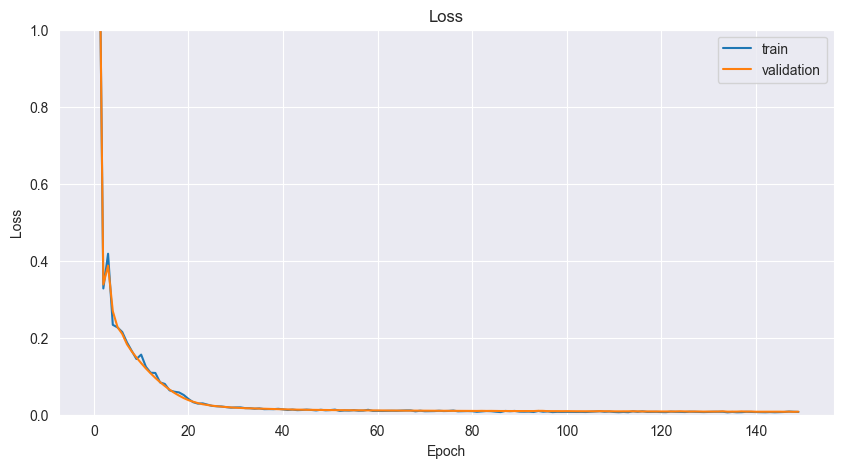
\includegraphics[width=.9\textwidth]{nn_loss.png}
    \centering
\end{figure}



\section{TabNet}
TabNet Results
\begin{table}[H]
    \centering
    \begin{tabular}{|c|c|c|c|}
        \hline
        \textbf{Model} & \textbf{MSE} & \textbf{RMSE}  & \textbf{MAE} \\
        \hline
        TabNet              & 0.00795749657941388   & 0.0892048013248944       & 0.0689039959039718    \\
        TabNet With PCA     & 0.00813222261181444  & 0.0901788368289059      & 0.964001783993923   \\
        \hline
    \end{tabular}
    
    \label{tab:tabnet_results}
\end{table}

\begin{table}[H]
    \centering
    \begin{tabular}{|c|c|}
        \hline
        \textbf{Model} &  \textbf{R2} \\
        \hline
        TabNet              & 0.964775228814175  \\
        TabNet With PCA     & 0.964001783993923  \\
        \hline
    \end{tabular}
    
    \label{tab:tabnet_resultsR2}
\end{table}

Miglior TabNet
\begin{table}[H]
    \centering
    \begin{tabular}{|c|c|c|c|c|}
        \hline
        \textbf{Batch Size} & \textbf{width}    & \textbf{step} & \textbf{lr}   & \textbf{Max Epochs}\\
        \hline
        2048                & 8     & 5 & 0.02  & 210   \\
        512 with PCA        & 32    & 5 & 0.02  & 150   \\
        \hline
    \end{tabular}
    
    \label{tab:best_tabnet}
\end{table}

Di seguito è riportato un grafico contenente l'andamento della funzione loss del training e validation del miglior modello di TabNet
\begin{figure}[H]
    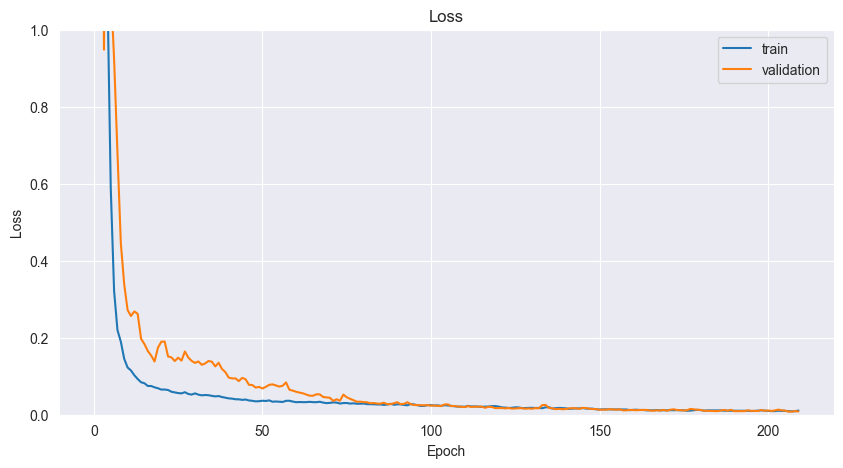
\includegraphics[width=.9\textwidth]{tabnet_loss.png}
    \centering
\end{figure}

\section{Conclusioni}
Nel presente lavoro si è eseguita la pipeline descritta nell'Introduzione, in seguito ad aver acquisito il dataset abbiamo addestrato i modelli sia con dati grezzi sia applicando la PCA confrontando i risultati.
Abbiamo notato che in tutti i modelli i risultati con PCA (n\_components = 0.95) hanno portato a una perdita di informazioni e non un risparmio in termini di tempo sostanziale.
Per tutti i modelli di Machine Learning è stato fissato il Random State per rendere possibile la riproducibilità dei risultati.
Il tuning degli iperparametri è stato effettuato con il metodo GridSearchCV con 3-fold cross validation per ottimizzare proprio il tempo ed avere un risultato congruo in termini di Mean Test Score tra tutti i modelli di Machine Learning.
Il modello dei Tabular Data è risultato molto più efficiente in termini di tempo rispetto alle Neural Network nonostante teniamo sempre in considerazione che i parametri (e di conseguenza i risultati) sono differenti.
Possiamo concludere che tutti i modelli (eccezzione fatta per KNN e DT) riescono a generalizzare bene sui dati in modo da fare previsioni accurate su dati mai visti in precedenza.
\end{document}


